\chapter{Progetto Interconnect}

Il progetto Interconnect ha l'obiettivo di introdurre concetti per l'interoperabilità e l'integrazione dei dati da diverse fonti, in modo che gli utenti possano fornire i propri servizi e accedere a informazioni pertinenti e correlate in modo più efficiente.


\section{Ontologie Interconnect}
Interconnect non è una singola ontologia, è una famiglia di ontologie che si basano sull'uso di ontologie già esistenti oltre a estendere SAREF e relative estensioni per l'energia.
Nella figura \ref{fig:panoramicaInterconnect} viene raffigurata una panoramica sulle ontologie create all'interno del progetto, mostrando le altre ontologie utilizzate ed estese. In particolare si può notare la famiglia SAREF di ETSI (SAREF e relative estensioni già trattate nel capitolo \ref{cap:panoramicaSaref}).
\begin{figure}[!ht]
    \centering
    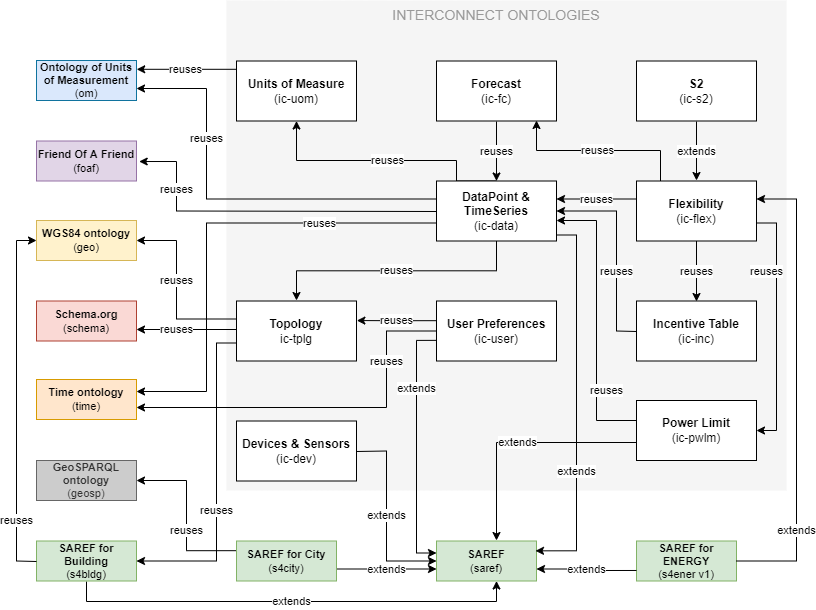
\includegraphics[width=\textwidth]{figures/panoramicaInterconnect.png}
    \caption{Panoramica delle ontologie InterConnect in relazione a SAREF e ad altre ontologie esistenti.}
    \label{fig:panoramicaInterconnect}
\end{figure}

\subsection{Ontologie create nel progetto Interconnect}

\subsection{Ontologie utilizzate}
L'utilizzo di altre ontologie è uno dei pilastri del web semantico. Nella tabella \ref{tab:ontologieUtilizzate} vengono elencate tutte le ontologie utilizzate nel progetto Interconnect, con relativo dettaglio sui concetti di tali librerie.
\begin{table}[htbp]
    \centering
    \begin{tabularx}{\textwidth}{|X|X|X|}
        \hline
        Prefisso & Namespace                                                               & Concetti                                                                            \\
        \hline
        foaf     & \href{http://xmlns.com/foaf/0.1/}{link}                                 & Agent                                                                               \\
        geo      & \href{http://www.w3.org/2003/01/geo/wgs84_pos}{link}                    & Spatial Thing, geo coordinates                                                      \\
        geosp    & \href{http://www.opengis.net/ont/geosparql}{link}                       & Geographical Feature                                                                \\
        schema   & \href{https://schema.org/}{link}                                        & Address, Countries, Postal Codes                                                    \\
        om       & \href{http://www.ontology-of-units-of-measure.org/resource/om-2/}{link} & Quantity, Unit, Measure                                                             \\
        saref    & \href{https://saref.etsi.org/core/}{link}                               & Device, Function, Command, State, Measurement, Unit of Measure, Feature of Interest \\
        s4bldg   & \href{https://saref.etsi.org/saref4bldg/}{link}                         & Building, Building Space, Building Object                                           \\
        s4city   & \href{https://saref.etsi.org/saref4ener/}{link}                         & Power Profile, Alternatives, Power Sequence, Slot                                   \\
        s4ener   & \href{https://saref.etsi.org/saref4city/}{link}                         & Facility, Administrative Area, City Object                                          \\
        time     & \href{http://www.w3.org/2006/time}{link}                                & Instant, Interval, Duration                                                         \\
        \hline
    \end{tabularx}
    \caption{Ontologie utilizzate all'interno del progetto Interconnect}
    \label{tab:ontologieUtilizzate}
\end{table}

\section{InterConnect Interoperability Framework}